%!TEX root = paper.tex
\section{Results}\label{sec:results}

Below we present first results from studying the aggregate
traffic across the multiple \gls{lorawan} gateways operated
by volunteers in the \gls{oin} community.
\todo[inline]{Daten von wann bis wann; wieviele Gateways und ungefähr wo; Spezifika der Sender, Empfänger hinsichtlich Kanälen, usw.}

\todo[inline]{Generelle Statistika, siehe auch notes.md}

\begin{figure}
  \centering
  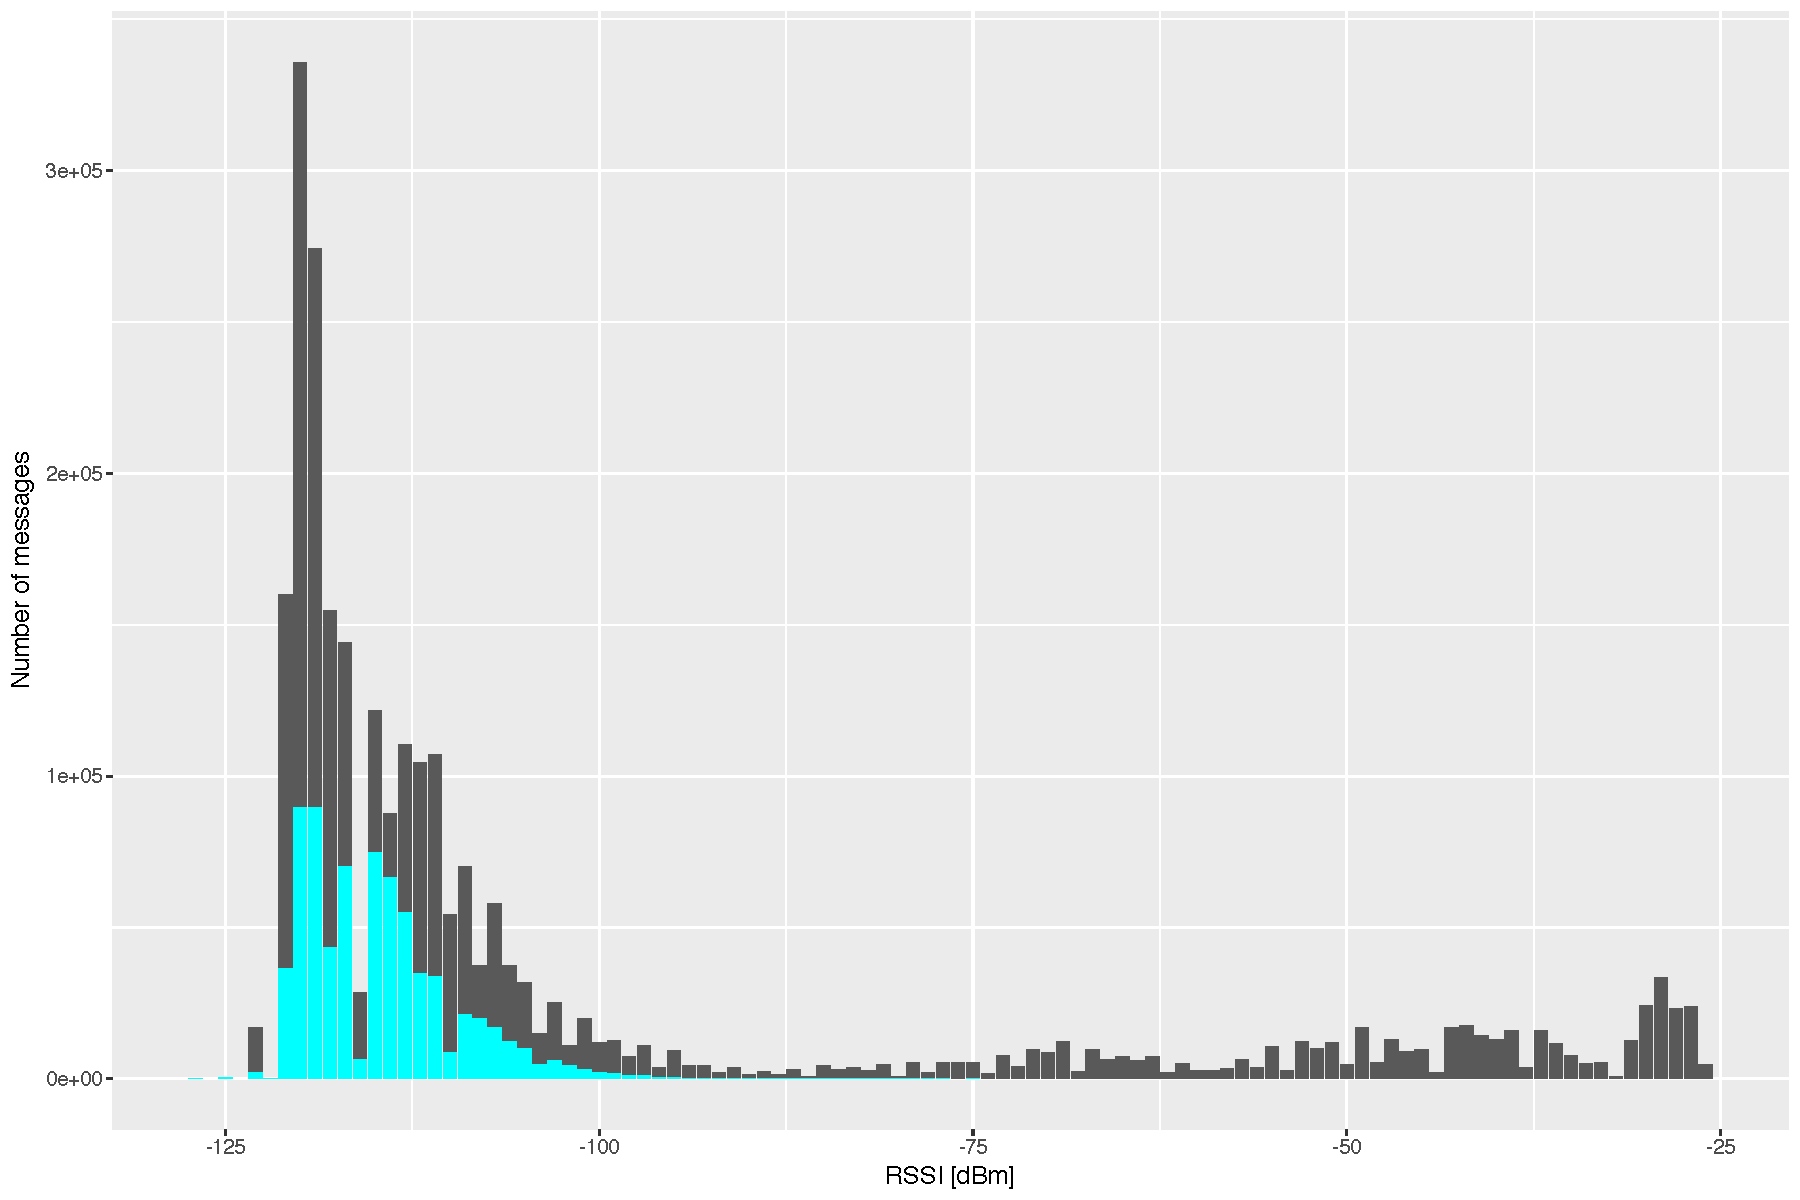
\includegraphics[width=\columnwidth]{figures/rssi.pdf}
  \caption{\acrshort{RSSI} for messages across all gateways (gray), and at the most active gateway (cyan).}
  \label{fig:rssi}
\end{figure}

Figure~\ref{fig:rssi} shows the \gls{RSSI} for messages across all
gateways (gray), and at the most active gateway (cyan).
\todo[inline]{keine geeichten Empfänger; wenig Leistung kommt an; Fading; Geografie der Empfänger; Geografie/Mobilität/nicht der Sender}




\begin{figure}
  \centering
  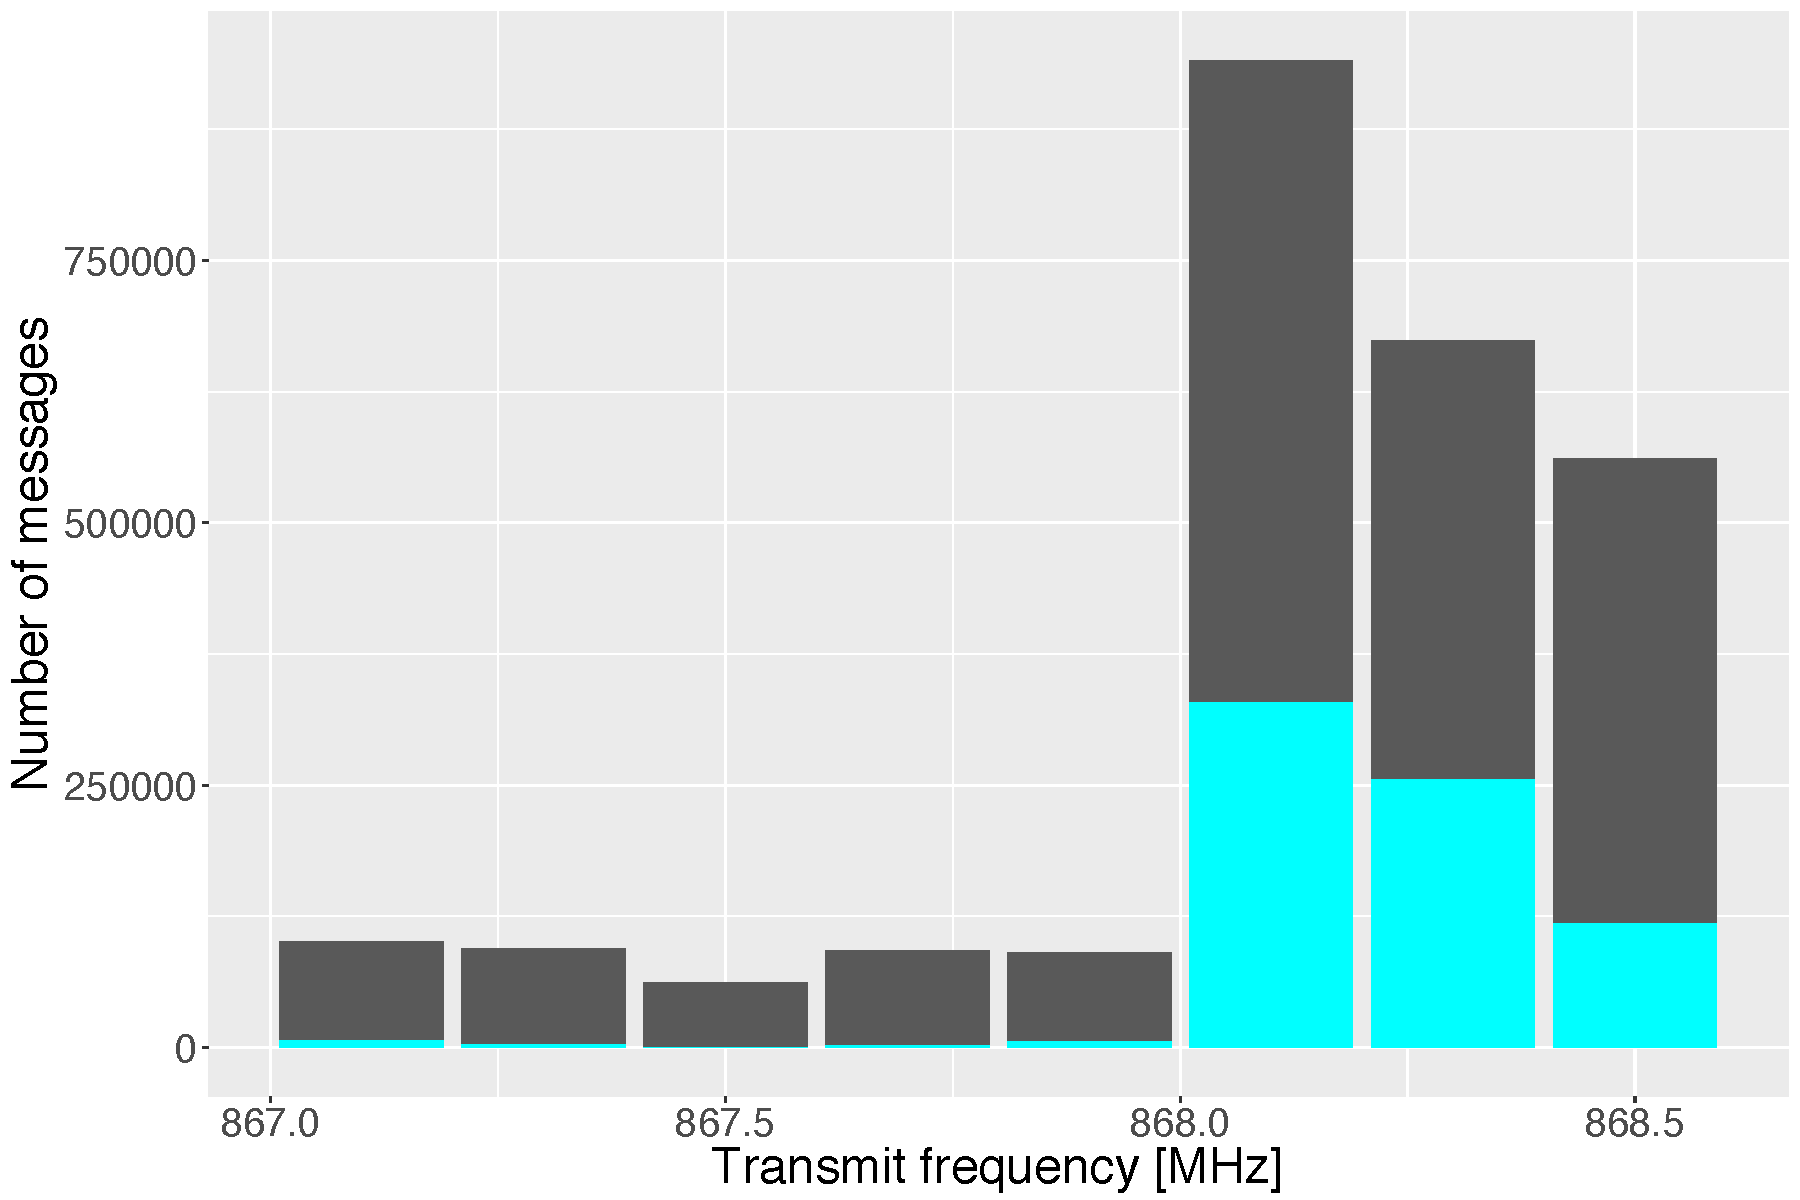
\includegraphics[width=\columnwidth]{figures/qrg.pdf}
  \caption{Transmission frequency for messages across all gateways (gray), and at the most active gateway (cyan).}
  \label{fig:qrg}
\end{figure}

Figure~\ref{fig:qrg} overviews the use of frequencies for transmissions
in the European \gls{SRD} band, as seen across all gateways (gray) and
at the most active gateway (cyan).
\todo[inline]{868,1 bis ,5 machen den Löwenanteil aus. Nicht alle Gateways können alle Frequenzen, und schon gar nicht alle Sender!}




\begin{figure}
  \centering
  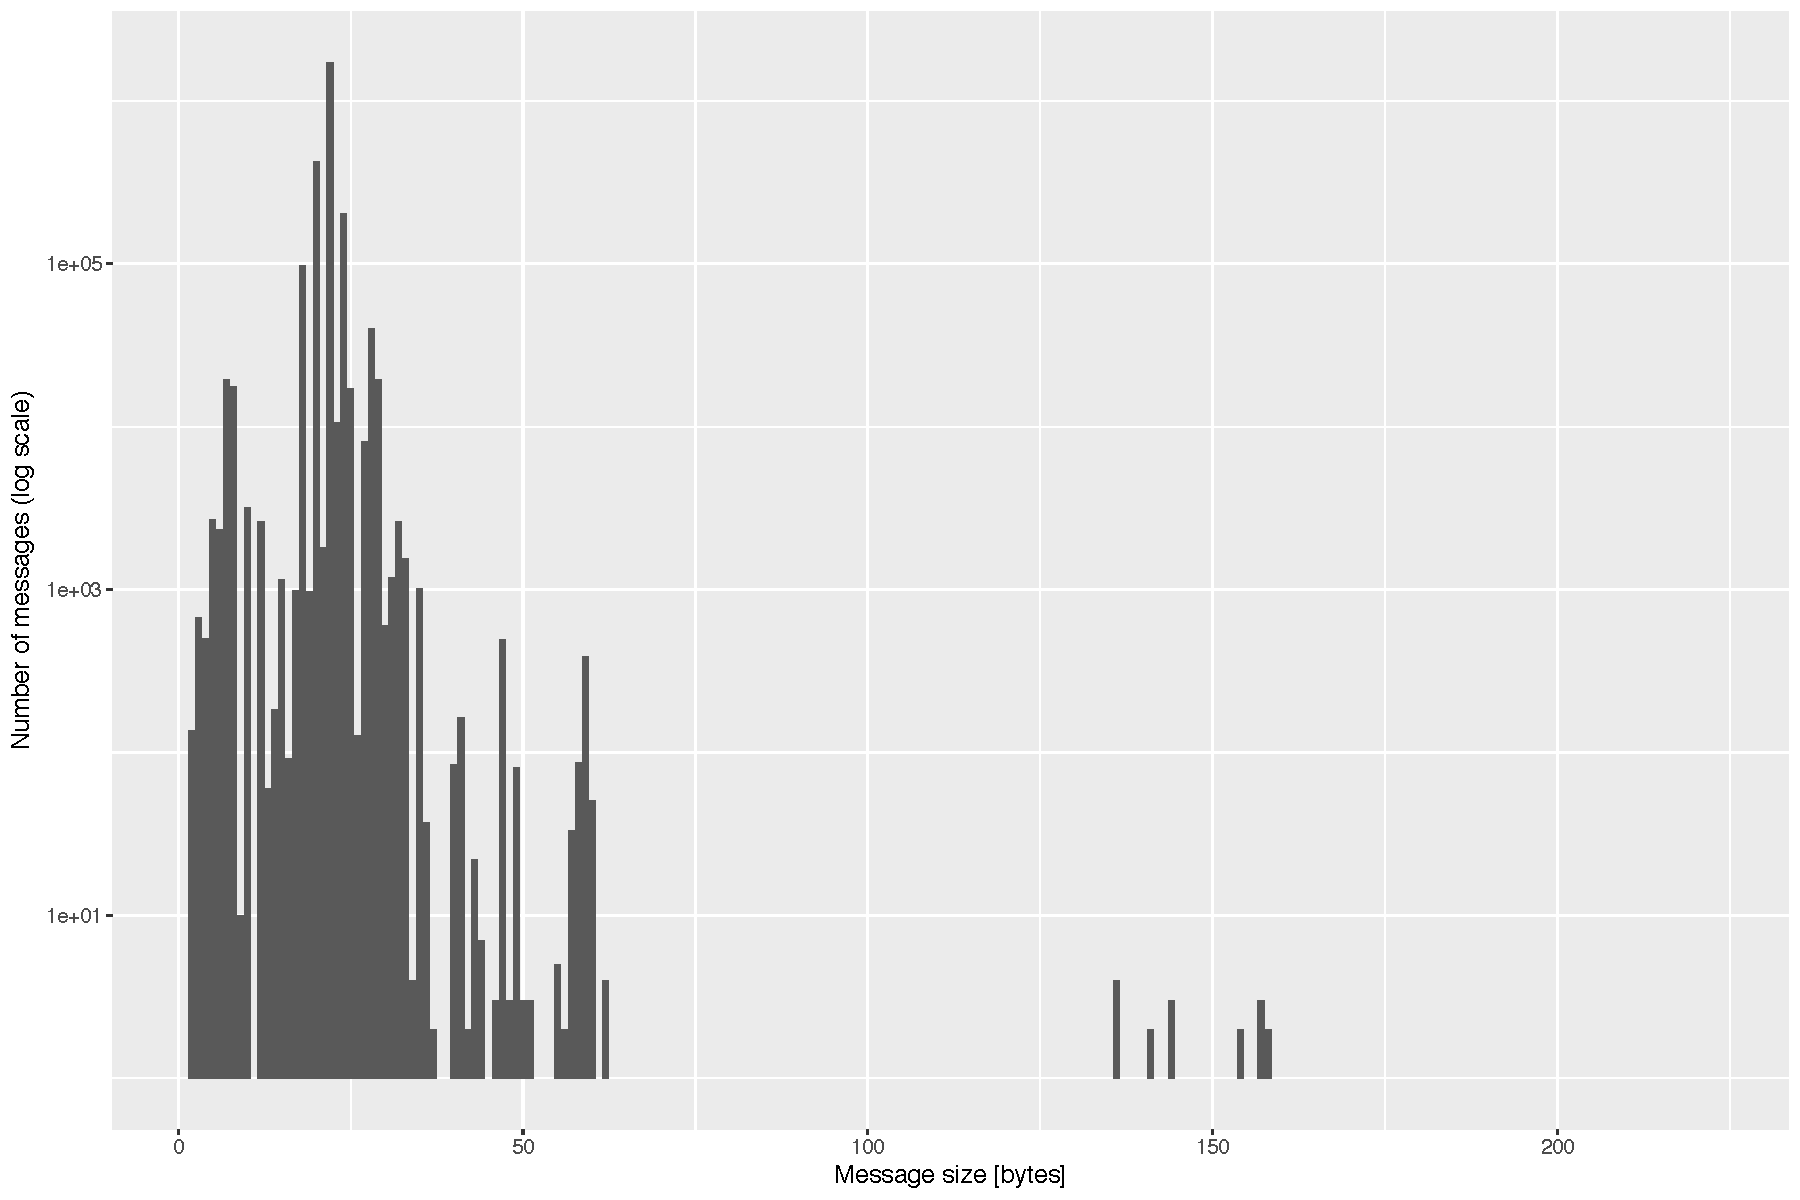
\includegraphics[width=\columnwidth]{figures/sizes.pdf}
  \caption{Message sizes across all gateways.}
  \label{fig:sizes}
\end{figure}

Figure~\ref{fig:sizes} plots the number of messages received across
all gateways, cumulated by message sizes. Note the logarithmic $y$ axis.
The mode of the distribution is $22$ bytes with a count of over 1.7 million.
A small cluster forms around the value.
\todo[inline]{Ein paar Spitzen (allerdings um Größenordnungen kleiner) gibt es noch; ohne detaillierten Blick in die Daten schwierig, weitere Schlüsse zu ziehen. Der prävalente SF12 ist immerhin kongruent mit kurzen Messages.}
